\chapter{Operating System}
\label{cha:operating-system}

\lstset{language=bash}

\section{CRLF}
\label{sec:crlf}

This sections talks about keys (and their names) and keybord.

We have \textit{physical} keyboard with labels like 1, 2, Enter,
Delete etc. The physically pressed keys are captured by OS and
then translated \textit{integer keycodes}. Programs read the
keycodes and interpret them as appropriate \textit{logical}
keys.

We can change keycodes passed from OS to a program like switching
left Ctrl and Caps. When Caps key is pressed, the Ctrl keycode is
sent to the program.

Several logical keys have their own names. Specifically, DEL, ESC,
LFD, SPC, RET, TAB, and \textit{newline} all stand for themselves
when seen in online posts. Name \verb|C-m| (pressing the
Return key) is translated to logical RET. \verb|C-k| for
pressing Control and \verb|k| simutaneously. \verb|C-j| is
translated to LFD. Don't be fooled. Logical name \verb|DEL|
corresponds to \verb|Backspace| on keyboard, not Delete.

Then let's have a look at ancient typewriter, comprising
\textit{Carriage Return} that helps feed a new line. When a new
line is required, the carriage return pulls back the typing head
and then a new paper line is fed up. So in the old times, a new
line consists of a Carriage Return and a Line Feed.

In the PC age, the corresponding keyboard key is Enter. When it is
pressed, the logical name is ENTER, also called
(\textit{electronical}) \textit{newline}. So it is not uncommon
that the Enter key has an arraw line as depicted in
\ref{fig:enter-return-key}. The vertical line means line feed
while the horizontal arrow means carriage return.

\begin{figure}
  \centering
  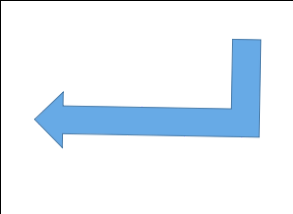
\includegraphics{return-enter-key}
  \caption{Enter/Return Key}
  \label{fig:enter-return-key}
\end{figure}

The two operations can be named as \verb|CR| and \verb|LF|
respectivelly. Programing languages, Bash included, use
\lstinline|\r| and \lstinline|\n| to denote the two names. In
Linux, it is \verb|\n|, while in Windows it is \verb|\r\n|. Mac
OS, to the contrary, is \verb|\r|. We call this \textit{line
  ending scheme}. It is critical to be aware of line ending
difference, especially when web techniques are involved like
\ref{lst:curl-crlf}.

\begin{itemize}
\item \verb|C-m, ^M, \r, Carriage Return, RET| are all the same
  thing.
\item \verb|C-j, ^J, \n, Line Feed, LFD| as well.
\end{itemize}

\section{Memory}
\label{sec:os-memory}

\subsection{Cost of Reclaiming}
\label{sec:cost-reclaiming}

The cost of memory \textit{initialization} and
\textit{destruction} of kernel data objects can actually outweigh
the cost of allocating them, which can result in significant
performance drop.

\begin{quotation}
  Kernel is reluctant to free up memory unless required.
\end{quotation}

\subsection{Slab Allocation}
\label{sec:slab-allocation}

A slab is a set of one or more \textit{continuous} memory pages
\textit{pre-allocated} for the slab allocator as an individual
\textit{cache}. This cache is further divided into \textit{equal
  segment}s (also called \textit{chunk} or \textit{slot}) in size
of the object type that the cache is managing. It is a memory
allocation mechanism intended for \textit{small} \uline{objects}
of the \textit{same type} like \textit{inode} and \textit{dentry}:

In this parlance, the word \uline{cache} or \uline{caching} refers
to a memory storage for a specific type of object, such as
\textit{semaphores}, \textit{process descriptors}, \textit{file
  objects}, etc. It is \textbf{not} the \textit{cache memory}
between the main memory and CPU.

A small object may be 8 bytes, 16 bytes, or 256 bytes large, but
usually far smaller than the size of a 4K memory page. If every
small object is allocated a separate memory page, it would be a
vast memory waste and
\href{https://stackoverflow.com/a/27762414}{lead to}
\textit{internal} and/or \textit{external} memory
\textit{fragmentation}.

\begin{landscape}
  The notion of \textit{object caching} was primarily introduced
  in order to \textit{avoid} the overhead such overheads.

  As a slab is pre-allocated, memory allocation request can be
  instantly satisfied in one of the preserved slot. Destruction of
  the object does not reclaim the slot but only puts the slot into
  the list of free slots by the slab allocator. This process
  eliminates the need to search for suitable memory space and
  greatly alleviates memory fragmentation.

  From file \lstinline|/proc/meminfo|, \uline{Slab} is the total
  amount of available slots. \uline{SReclaimable} can be freed up
  by kernel for other usage while \uline{SUnreclaim} cannot.

  For slab details, execute \lstinline|man 5 slapinfo| and
  \lstinline|slabtop|. Here is an excerpt \ref{lst:slab-info}:

\begin{lstlisting}[caption={Slab Info},label={lst:slab-info},basicstyle=\tiny\ttfamily]
# name               <active_objs> <num_objs> <objsize> <objperslab> <pagesperslab> : tunables <limit> <batchcount> <sharedfactor> : slabdata <active_slabs> <num_slabs> <sharedavail>
ext4_groupinfo_4k    364    364    144   28    1 : tunables    0    0    0 : slabdata     13     13      0
squashfs_inode_cache      0      0    640   25    4 : tunables    0    0    0 : slabdata      0      0      0
fuse_inode          3864   3864    768   21    4 : tunables    0    0    0 : slabdata    184    184      0
PINGv6                 0      0   1152   28    8 : tunables    0    0    0 : slabdata      0      0      0
RAWv6                 56     56   1152   28    8 : tunables    0    0    0 : slabdata      2      2      0
tw_sock_TCPv6          0      0    240   17    1 : tunables    0    0    0 : slabdata      0      0      0
request_sock_TCPv6      0      0    304   26    2 : tunables    0    0    0 : slabdata      0      0      0
dma-kmalloc-16         0      0     16  256    1 : tunables    0    0    0 : slabdata      0      0      0
dma-kmalloc-8          0      0      8  512    1 : tunables    0    0    0 : slabdata      0      0      0
dma-kmalloc-192        0      0    192   21    1 : tunables    0    0    0 : slabdata      0      0      0
kmalloc-8192          72     72   8192    4    8 : tunables    0    0    0 : slabdata     18     18      0
kmalloc-4096         249    272   4096    8    8 : tunables    0    0    0 : slabdata     34     34      0
kmalloc-512          864    912    512   16    2 : tunables    0    0    0 : slabdata     57     57      0
\end{lstlisting}

  The first column is the \textit{names} of different types of
  slabs. \textit{kmalloc-512} means this slab is designated for
  512-byte objects. So is \textit{dma-kmalloc-192} for 192-byte
  objects. To filter slabs larger than or equal to 10M, run:

\begin{lstlisting}
awk '{ if ( $3*$4/1024/1024 > 10 ) { print $1, $3*$4/1024/1024 } }' /proc/slabinfo
\end{lstlisting}

\end{landscape}

%%% Local Variables:
%%% mode: latex
%%% TeX-master: "main"
%%% End:
